\section{Experiments}
\label{sec:experiments}




In this section, we perform preliminary simulations to demonstrate the ICRL capabilities of transformers and validate our theoretical findings. We remark that while similar experiments have been conducted in existing works~\citep{laskin2022context,lee2023supervised}, our setting differs in several aspects such as imitating the entire interaction trajectory in our pretrain loss~\eqref{eq:general_mle} as opposed to on the last (query) state only as in~\citet{lee2023supervised}. The code is available at~\href{https://github.com/licong-lin/in-context-rl}{https://github.com/licong-lin/in-context-rl}.




We compare pretrained transformers against empirical average, LinUCB (or UCB), and Thompson sampling. We use a GPT-2 model~\cite{garg2022can,lee2023supervised} with $L = 8$ layers, $M=4$ heads, and embedding dimension $D=32$. We utilize ReLU attention layers, aligning with our theoretical construction. We pretrain the transformer with two setups: (1) Both context algorithm $\sAlg_0$ and expert algorithm $\sAlg_{\shortexp}$ use LinUCB (the Algorithm Distillation approach); (2) Context algorithms $\sAlg_0$ mixes uniform policy and Thompson sampling, while expert $\sAlg_{\shortexp} = \action_t^*$ provides optimal actions (DPT). See Appendix \ref{sec:exp_details} for further experimental details.


In the first setup, we consider stochastic linear bandits with $d=5$ and $A=10$. At each $t \in [200]$, the agent chooses an action $\action_t$ and receives reward $\reward_t=\<\action_t,\bw^*\>+\eps_t$ where $\eps_t\sim\cN(0,1.5^2)$. The parameter $\bw^*$ is from ${\rm Unif}([0,1]^d)$. The action set $\sA_t=\sA$ is fixed over time with actions i.i.d. from ${\rm Unif}([-1, 1]^d)$. We generate 100K trajectories using $\sAlg_0=\sAlg_{\shortexp}=\LinUCB$ and train transformer $\TF_\EstPar(\cdot)$ via Eq.~\eqref{eq:general_mle}. Figure~\ref{fig:regret_1} (left) shows regrets of the transformer (TF), empirical average (Emp), LinUCB, and Thompson sampling (TS). The transformer outperforms Thompson sampling and empirical average, and is comparable to LinUCB, agreeing with Theorem~\ref{thm:smooth_linucb}. The small regret gap between TF and LinUCB may stem from the limited capacity of the GPT2 model.




In the second setup, we consider multi-armed Bernoulli bandits with $d = 5$. The parameter $\bw^*$ is from ${\rm Unif}([0,1]^d)$. The fixed action set $\sA_t=\sA$ contains one-hot vectors $\{\be_i\}_{i=1}^d$ (multi-armed bandits). At each $t \in [200]$, the agent selects $\action_t$ receives reward $r_t \sim {\rm Bern}(\<\action_t,\bw^*\>)$. Let $\sAlg_{\mathrm{unif}}$ be the uniform policy. We use $\sAlg_{\mathrm{unif}}$ and $\sAlg_\TS$ as context algorithms to generate $50$K trajectories each. The expert is fixed as $\sAlg_\shortexp=\action^*$. We train transformer $\TF_\EstPar(\cdot)$ via Eq.~\eqref{eq:general_mle}. Figure~\ref{fig:regret_1} (right) shows regrets for the pretrained transformer (TF), empirical average (Emp), UCB, and Thompson sampling (TS).  The transformer aligns with Thompson sampling, validating Theorem~\ref{thm:ts_linear_regret}. However, TS underperforms UCB for Bernoulli bandits, as shown.





\begin{figure}[t]
\centering  %
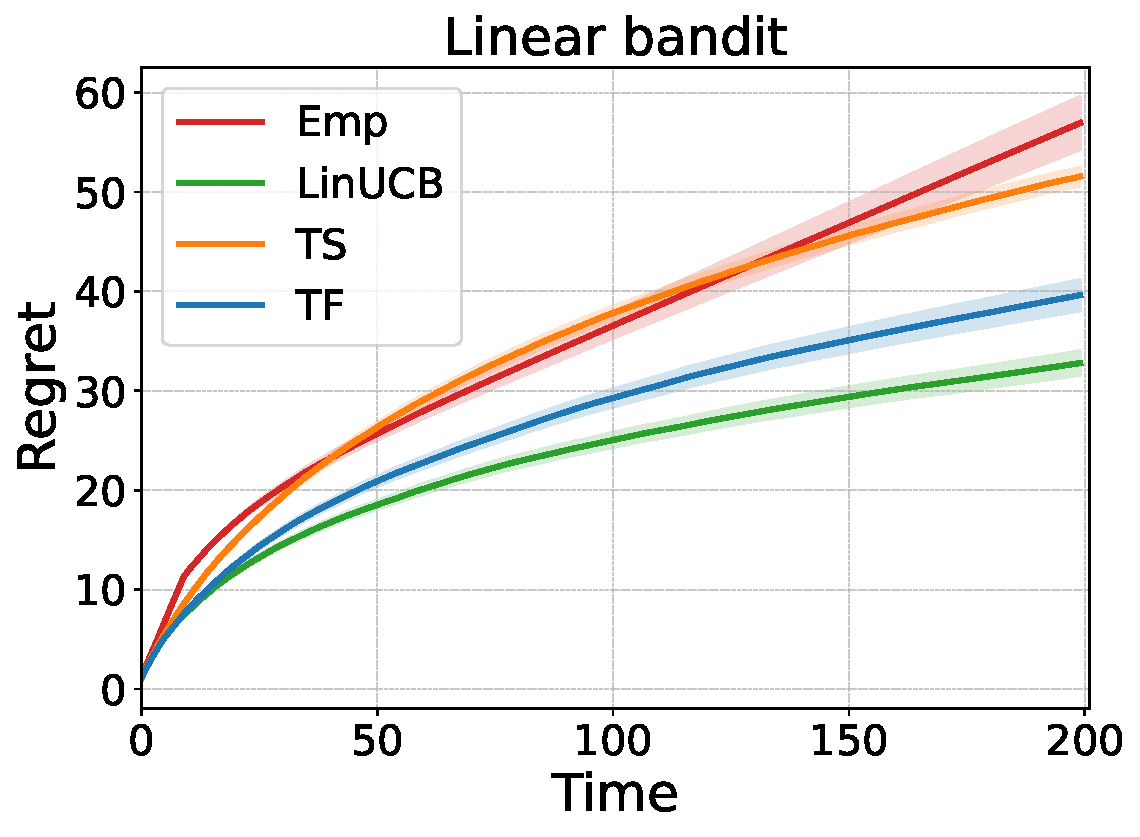
\includegraphics[width=0.35\linewidth]{Sections/figs/record_2_cum_True.pdf}
\hspace{2em}
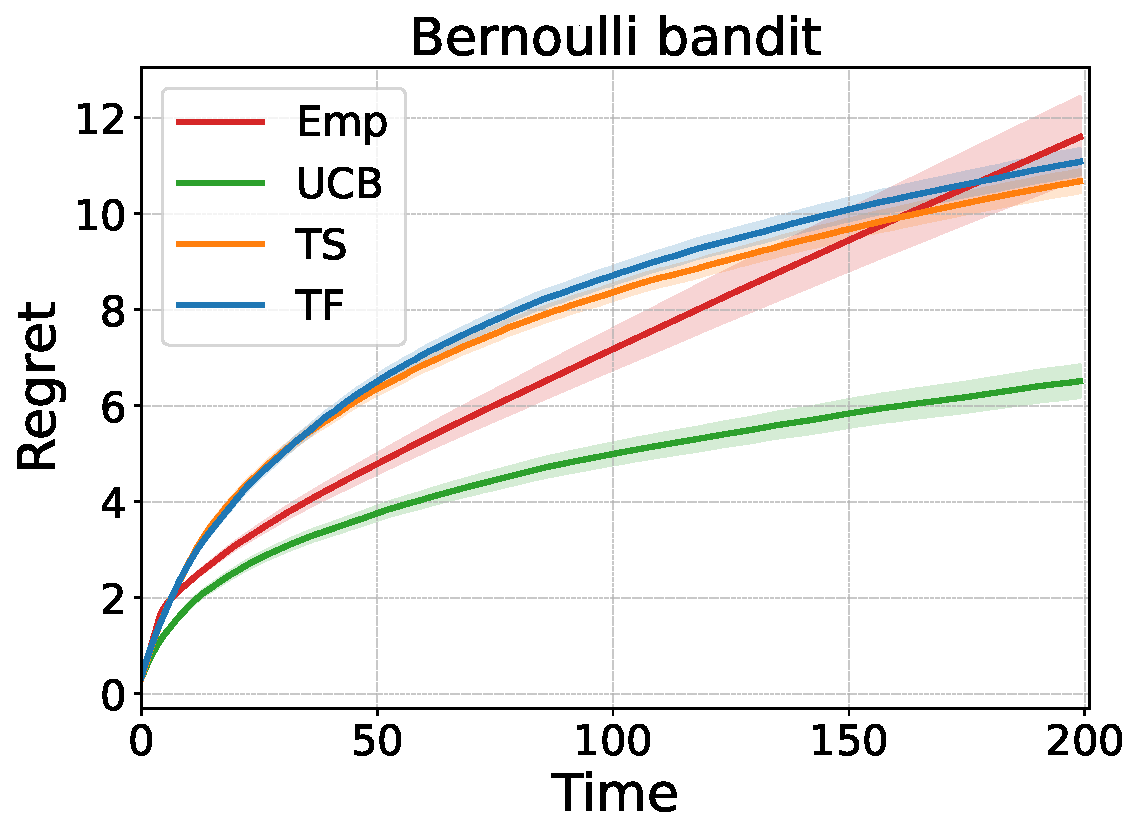
\includegraphics[width=0.35\linewidth]{Sections/figs/record_1_cum_True.pdf}
\vspace{-1em}
\caption{Regrets of transformer (TF), empirical average (Emp), Thompson sampling (TS) and LinUCB or UCB (LinUCB reduces to UCB for Bernoulli bandits). Left: linear bandit with $d=5$, $A=10$, $\sigma=1.5$, $\sAlg_0=\sAlg_\shortexp=\LinUCB$. Right: Bernoulli bandit with $d=5$, $\sAlg_0=(\sAlg_{\mathrm{unif}}+\sAlg_{\TS})/2$ and $\sAlg_\shortexp=\action^*$. The simulation is repeated 500 times. Shading displays the standard deviation of the regret estimates. }
\label{fig:regret_1}
\end{figure}

